\documentclass[../main.tex]{subfiles}
 
\begin{document}

% ---------------------------------------------------
% METODOLOGIA                                        
% ---------------------------------------------------
\chapter{Metodologia}

Neste capítulo é apresentada a metodologia de desenvolvimento da solução proposta. Para melhor entendimento, a metodologia está dividida em cinco etapas. Nas seções abaixo cada etapa será descrita detalhadamente.

\begin{figure}[h]
\centering
\caption{Etapas do Processo KDD.}
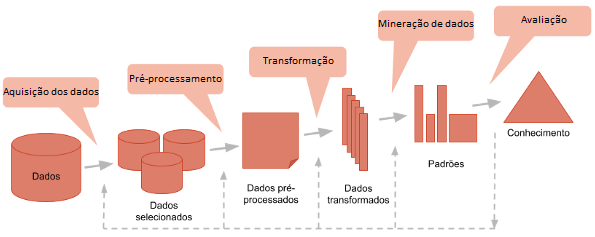
\includegraphics[width=1\textwidth]{Images/kdd.png}
\legend{\small Fonte: Adaptado de \cite{karinamoura}.}
\label{fig:Digitos_analogicos}
\end{figure}
 
 
\section{Aquisição dos dados}

Nesta etapa, espera-se que a base possua informações de consumo de cliente e dados temporal, que podem ser adquiridos dos mais diversos setores da companhia de energia elétrica. Pois, é possível que as informações essenciais a cerca do perfil de um cliente estejam separadas em vários domínios e banco de dados de vários setores de uma concessionária de energia.


\section{Pré-processamento}
O pré-processamento é uma etapa essencial no trabalho, pois a condição dos dados define a eficácia dos algorítimos de mineração. Nesta parte serão utilizadas técnicas para eliminar dados inconsistentes e redundantes, e que permitam encontrar possíveis dados divergentes ao conjunto.

Neste estágio, do mesmo modo, são utilizados métodos de transformação ou redução para diminuir o número de variáveis envolvidas no processo, com o intuito de  aperfeiçoar a performance   dos   algoritmos   de predição.

\section{Transformação}
Após a etapa de pré-processamento os dados precisam ser formatados adequadamente para que os algoritmos de séries temporais possam ser aplicados. Para este fim, será utilizado o \textit{framework} \textit{Featuretools}\footnote{Featuretools - An open source python framework for automated feature engineering, disponível em: https://www.featuretools.com/}, que é uma ferramenta automatizada para engenharia de características, com o objetivo de transformar os dados adquiridos em características temporais para a criação do modelo de predição.


\section{Mineração de dados}

A mineração de dados é o processo pelo qual se explora e analisa, de forma automática ou semi-automática, a partir de grandes bases de dados com o objetivo de encontrar padrões e regras \cite{han2011data}. Assim, nesta etapa, serão utilizados para as predições do perfil temporal do consumidor algorítimos de séries temporais assim como técnicas de classificação para determinar se um cliente irá ou não entrar com uma ação judicial.

As técnicas de classificação utilizadas serão \textit{Long-Short Term Memory (LSTM)}, \textit{Extreme Gradient Boosting (XGBoost)}, \textit{Logistic Regression (Regressão Logítica)} , \textit{Random Forest}, \textit{Support Vector Machine (SVM)} e para as séries temporais será utilizada a Análise de sobrevivência, do inglês: \textit{Survival Analysis}.




\section{Avaliação}
Ao fim do trabalho, os resultados obtidos através da solução elaborada com as técnicas de séries temporais serão avaliados nas métricas \textit{Mean Absolute Error} (MAE); \textit{Mean Absolute Percentage Error} (MAPE), Erro Percentual Absoluto Médio; \textit{Root Mean Square Error} (RMSE). Além disso, serão utilizadas métricas comumente usadas em problemas de classificação binária como a acurácia (AC), precisão (PRE), sensibilidade (SEN) e especificidade (ESP).

  
\end{document}
